\chapter{Ovládání jednotlivých elektronických částí}
\label{4-algoritmus}

\section{PWM}
Pro komunikaci regulátorů otáček a ovládání motorů je nutné znát pulzně šířkovou modulaci. Tato podkapitola stručně popíše princip  a funkci PWM.\\
PWM modulace je určená pro přenos analogového signálu pomocí dvou hodnot (Low a High), přenos probíhá na digitálních pinech. Přenášená hodnota je zaimplementováná do poměru High/Low. Poměru se nazývá střída a nabývá hodnot 0-100 procent. Hodnoty Low a High se zapisují v cyklu. Pro příjem signálu je důležité znát frekvenci cyklu, aby mohlo dojít k dekódování a určení zaslané hodnoty.

%http://1oomzzme3s617r8yzr8qutjk-wpengine.netdna-ssl.com/wp-content/uploads/2017/04/Fig-1-pwm.gif
\begin{figure}[h]
	\centering
	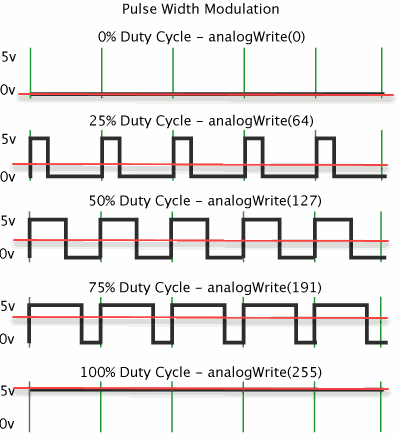
\includegraphics[width=10cm]{pictures/pwm.png}
	\caption{Ukázka PWM}
\end{figure}


\section{Kalibrace regulátorů otáček}
%https://www.youtube.com/watch?v=61bjFxJyOLU&t=52s

Pro kalibraci je potřeba kalibrovaný regulátor, propojovací dráty a Arduino Nano. V programu BLHeliSuite lze kalibrovat i s jinou platformu Arduino, bohužel kalibrace se podařila pouze s Arduino Nano.\\
Zapojení regulátoru se proveve přes schéma na obrázku.\\
Po zapojení komponent a nastavení šablony se vybere seriový port pro komunikaci mezi počítačem a Arduinem. Přes tlačítko Read Setup se načte tovární nastavení regulátoru.\\
 Nastaví se PPM Min Throttle hodnota na 1000, PPM Max Throttle na 2000 a PPM Center Throttle na 1500. Zapíše se hodnota do regulátoru. Doporučuji znovu zkontrolovat, někdy se stalo, že hodnoty se nenahrály. Tím se zkalibrovali vstupní hodnoty časování pulzu do intervalu 1000;2000. \\
Při každém zapnutí motoru je potřeba kalibrace a to posláním příkazu s hodnotou Min Throttle a následně Max Throttle.


\begin{figure}[h]
	\centering
	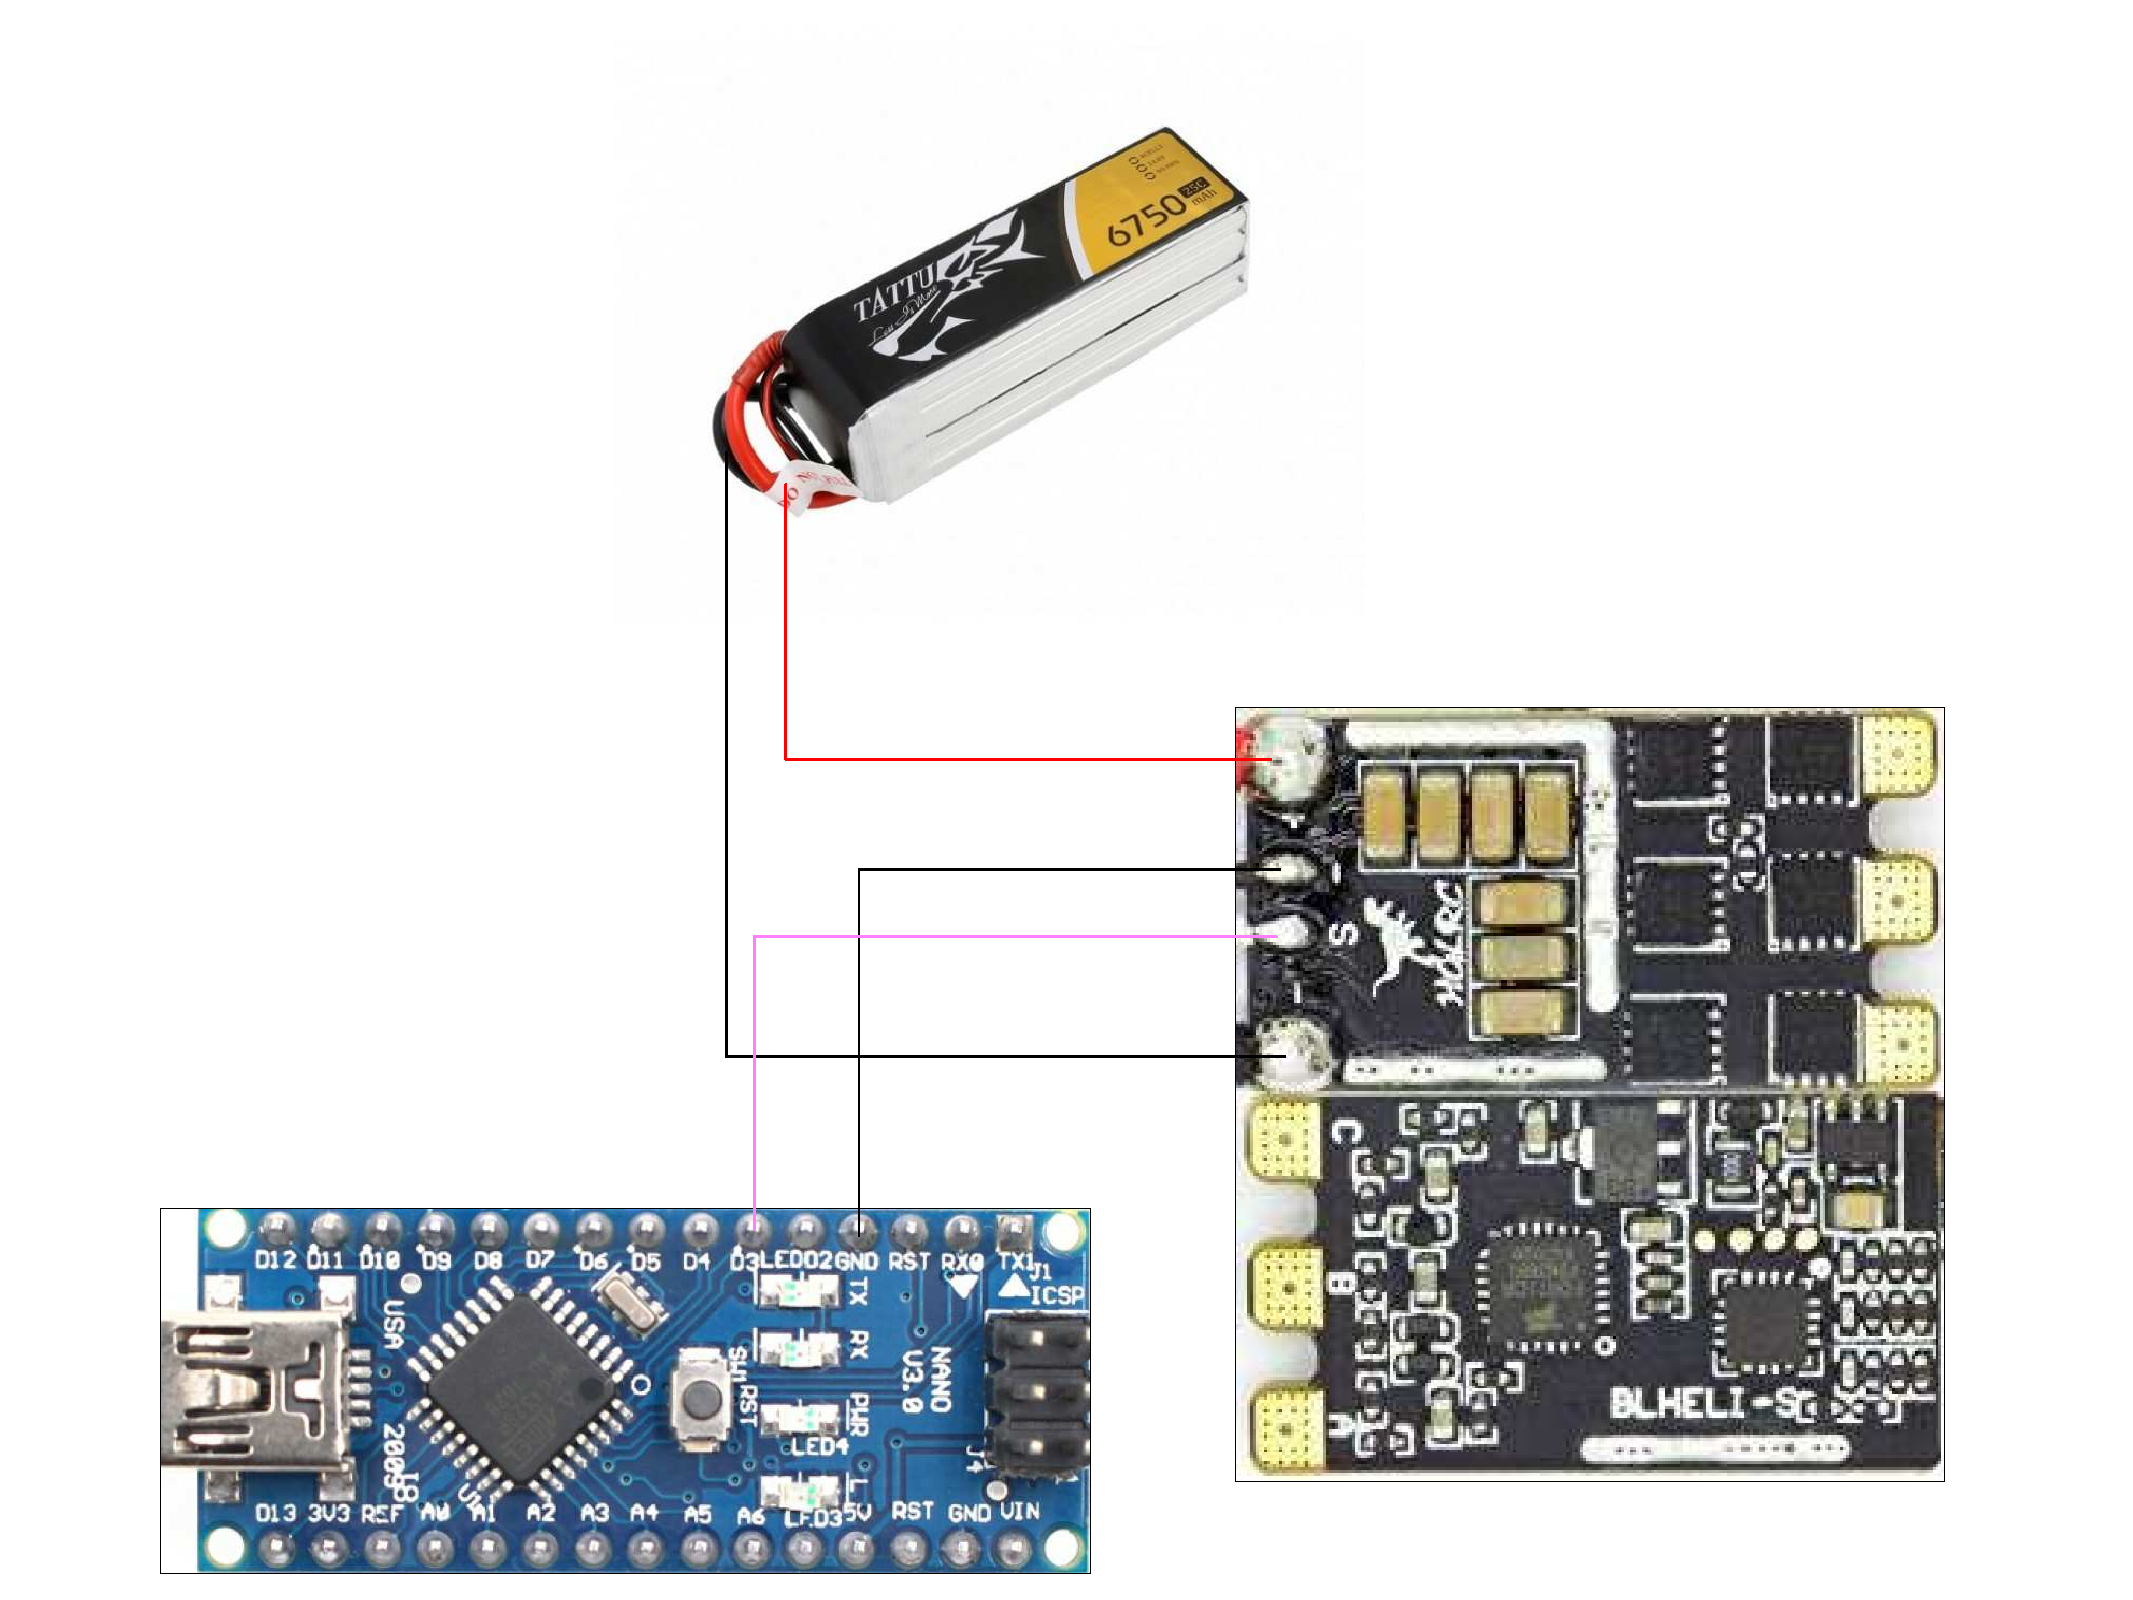
\includegraphics[width=12cm]{pictures/esc_calib.pdf}
	\caption{Schéma zapojení pro kalibraci regulátoru otáček}
\end{figure}

%https://www.youtube.com/watch?v=61bjFxJyOLU&t=52s

\section{Filtrace dat IMU}
Surová data ze všech tří senzorů nejsou samostatně použitelná pro ovládání drona. Surová data obsahují nepřesnosti a šum, proto je potřebná filtrace, ze které dostaneme úhly pitch, roll a yaw.
Surová data z IMU lze filtrovat různými způsoby.

%https://aip.scitation.org/doi/pdf/10.1063/1.5018520

\subsection{Komplementární filtr}
Komplementární filtr je nejjednodušší z uvedených filtrů. Využívá data z akcelerometru a gyroskopu. \\
Data z gyroskopu jsou unášena v čase, tedy když gyroskop je v klidu, měřená data se mění integračně. Z krátkodobého hlediska data z gyroskopu jsou přesná, proto pro další použití je potřeba použít High Pass filtr.\\
Opakem toho jsou data z akcelerometru, data jsou ovlivnováná malými silami, které ruší výsledné zrychlení. Z dlouhodobého hlediska jsou data z akcelerometru přesná, proto je potřeba použít Low Pass filtr.\\
Kombinací High Pass filtru a Low Pass filtr vzniká komplementární filtr, který pro použití při stavbě drona je dostačující.\\

\subsection{Kalmanův filtr}
Kalmanův filtr je dynamický filtr, který pracuje s predikcí. Pro výpočet je potřeba stanovit model systému, u kterého bude filtr predikovat stavy. Pokud v oblasti predikovaného stavu najdeme skutečný stav, provede se korekce skutečného stavu a oblast predikovaného stavu bude menší/přesnější. Nenalezne-li se v oblasti predikovaného stavu skutečný stav, oblast se zvětší/zhorší se přesnost.\\
Bohužel Kalmanův filtr nemohl být použít z důvodu malé výpočetní síly platformy Arduino.

\subsection{Mahonyho filtr}
Mahonyho filtr využívá Quaternions, což je čtyř dimensonální numerický systém využívaný pro popis rotace objektu v počítačové grafice a robotice. Filtr používá data z gyroskopu, akcelerometru a magnetometru, přičemž z nich počítá úhly pitch, roll a yaw.Při výpočtu použita knihovna MahonyAHRS.\\
%https://github.com/PaulStoffregen/MahonyAHRS
%https://www.youtube.com/watch?v=zjMuIxRvygQ

\section{PID regulátor pro synchornizaci motorů} 
Proportional Integral Derivative
PID regulátor slouží k regulaci požadovaného stavu za co nejkratší dobu a to za pomocí zvyšování a snižování vlivu, který napomáhá se dostat do požadovaného stavu.\\
Názorný příklad:
Chceme aby dron dokázal balancovat, chceme tedy aby proměné pitch a roll z IMU byly nulové. Kdybychom měli ideálního drona s přesným vyvážením hmotnosti a se stejně fungujícími motory, bylo by to snadné. Pouze by stačilo zapsat stejnou hodnotu na všechny motory a dron by bez problémů vzlétnul. Bohužel ideálního drona nemáme, proto musíme motory ovládat individuálně.\\
PID regulátor reaguje na tzv. errory (odchylky od požadovaného stavu) a následně přes koeficienty kp, ki a kd spočte hodnoty pro ovládání motorů.
PID regulátor má tři složky: proporcionální, integrační a derivační.\\
Proporcionální složka ovlivnuje ovládání motorů lineárně. Pokud je odchylka veliká zvýší se rychlost na motorech, pokud je odchylka nulová, motory se plně zastaví a spustí se až když je odchylka není nulová.\\
Integrační složka ovlivnuje ovládání motorů v závislosti na předchozím stavu. Pokud je odchylka velká, integrační složka se zvětšuje do doby dokud nepřesáhne požadovaný stav, potom se integrační složka zmenšuje a mění svoje znaménko.\\
Derivační složka reaguje na změnu rychlosti odchylky. Čím rychleji se bude zvyšovat odchylka tím rychleji se bude zvětšovat rychlost na motorech. Deriviční složka reaguje proti P a I složce.\\
Pro stabilizaci drona budou odchylky představovat náklony pitch and roll s opačným znaménkem. Po vyčíslení proporciální, integrační  a derivační složky, se nastaví rychlost jednotlivých motorů.

\begin{figure}[h]
	\centering
	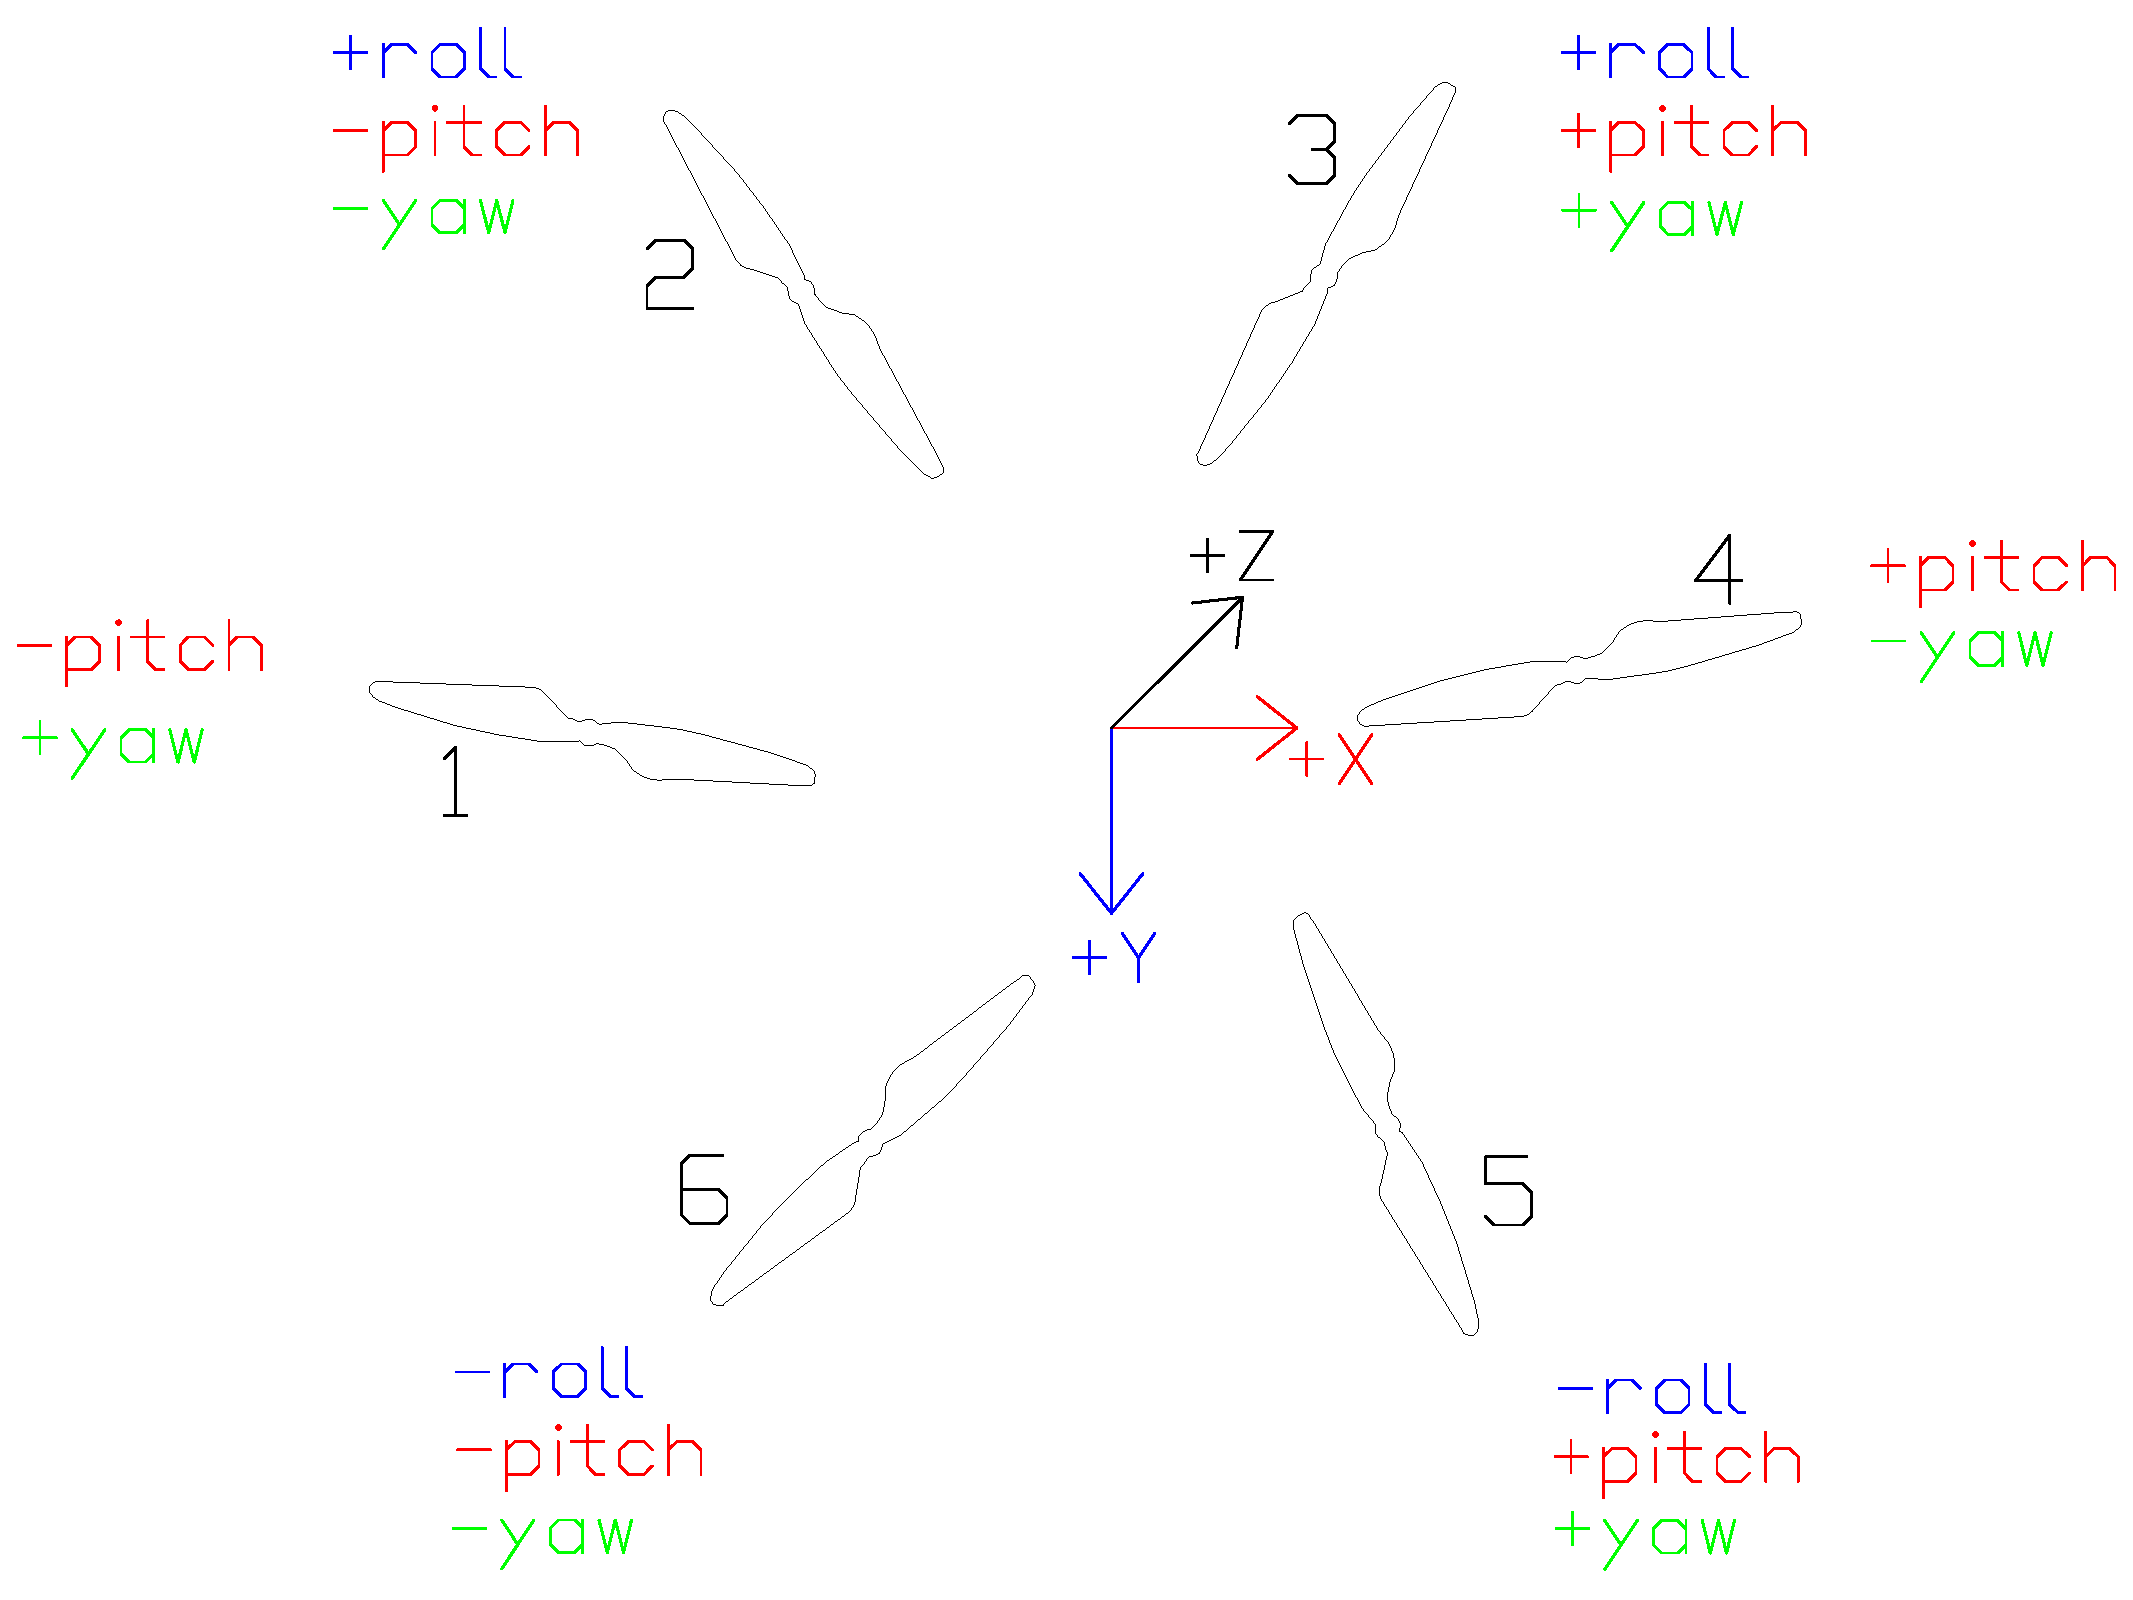
\includegraphics[width=12cm]{pictures/pid.pdf}
	\caption{Schéma ovládání vrtulí podle úhlu náklonu}
\end{figure}
%https://valter.byl.cz/plynula-regulace-pid
%http://www.controlengcesko.com/hlavni-menu/artykuly/artykul/article/derivacni-slozka-v-regulaci-pid/

\begin{figure}[h]
	\centering
	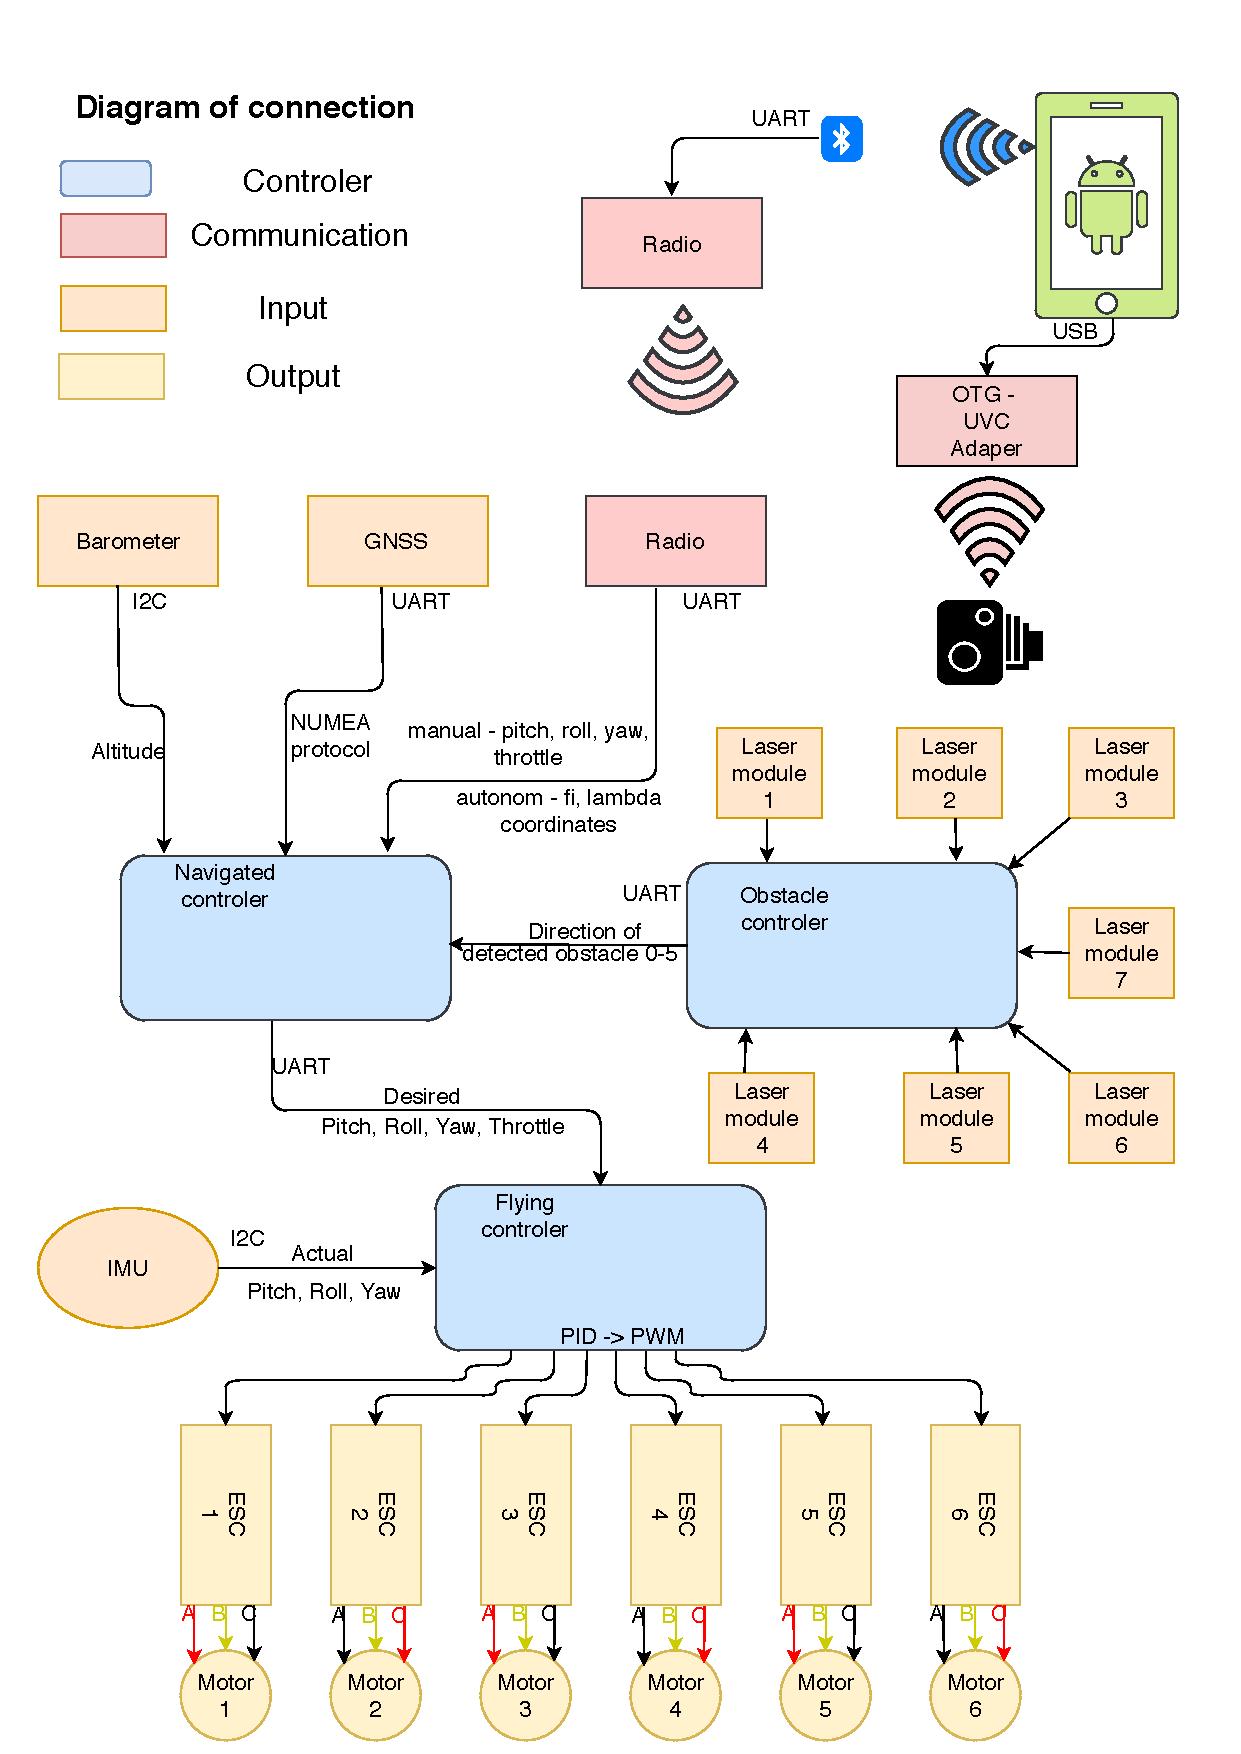
\includegraphics[width=15cm]{pictures/DroneDiagram.pdf}
	\caption{Diagram komponent}
\end{figure}

\section{Létající kontrolér} 
Vstup: IMU, Navigační kontrolér\\
Výstup: ESC\\

Létající kontrolér slouží k synchornizaci a ovládání motorů drona. Létající kontrolér zpracovává měření z IMU a porovnává jej s daty z navigačního kontroléru (pitch, roll a yaw). Pokud úhly náklonů nejsou totožné, kontrolér přes PID regulátor změní rychlost motorů, tak aby úhly ztotožnil.\\
Při spuštění létající kontrolér provede kalibraci regulátorů otáček tím, že zapíše minimální a maximální hodnotu výkonu.\\
Po proběhnutí kalibrace reguláorů otáček, čte data z IMU, fitruje je přes Mahonyho filtr a počítá pitch, roll a yaw. Uhly jsou použitelné po jedné minutě, potom je možné ovládat motory.\\
Z navigačního kontroléru jsou získávána data, která jsou násedně separována a interpolována do požadových hodnot. Hodnoty se rozlišují prvním bytem, který je písmeno definující o jakou hodnotu se jedná. Další dva byte definují číslo od 0 do 99, které se vyinterpoluje na požadovaný rozsah.\\

\begin{tabbing}
	Zprava ~ \= uhel ~~~~~~~~~ \= od ~~~~~~~ \= do ~~~~
	\= 34 \kill
	\bfseries Byte \>
	\bfseries Zpráva \>
	\bfseries Od \>
	\bfseries Do \\
	T\> Throttle \> 1000 uS \> 1700 uS \\
	P\> Pitch \>  -25$^\circ$ \> +25$^\circ$   \\
	R\> Roll \> -25$^\circ$ \> +25$^\circ$ \\
	Y\> Yaw \> 0$^\circ$ \> 360$^\circ$ \\
\end{tabbing}

Hodnota výkonu motoru/throttle se vyinterpoluju jenom do 1700, protože k hodnotě se ještě přičítá údaje z PID regulátoru. Pokud bychom zapsali hodnotu vyšší než 2000 spálil by se regulátor otáček.\\
Hodnota náklonů pitch a roll  může být nejvýše 25 stupňů, kdyby byla hodnota větší hrozilo by přerácení dronu.\\

\begin{figure}[h]
	\centering
	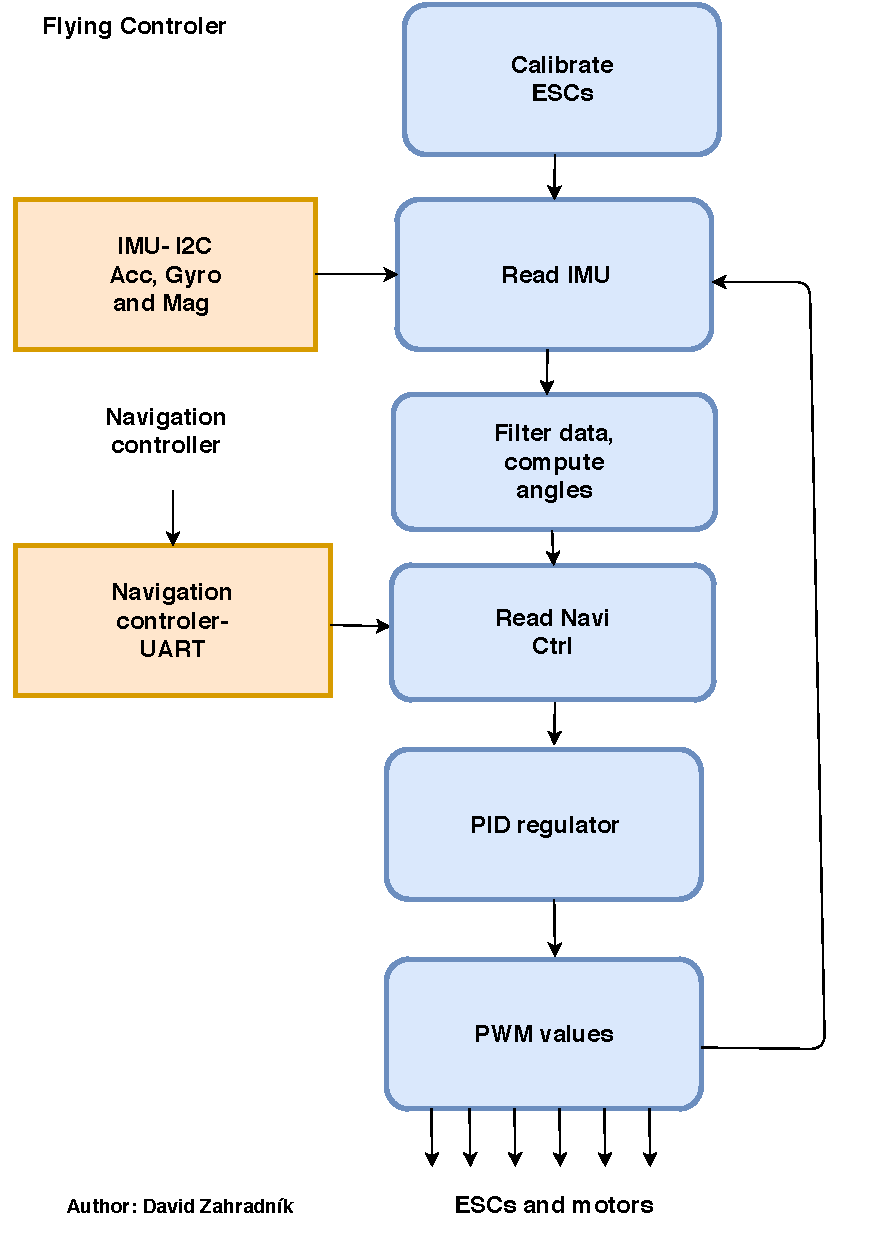
\includegraphics[width=15cm]{pictures/FlyingDiagram.pdf}
	\caption{Diagram algoritmu létajícího kontroléru}
\end{figure}


\begin{figure}[h]
	\centering
	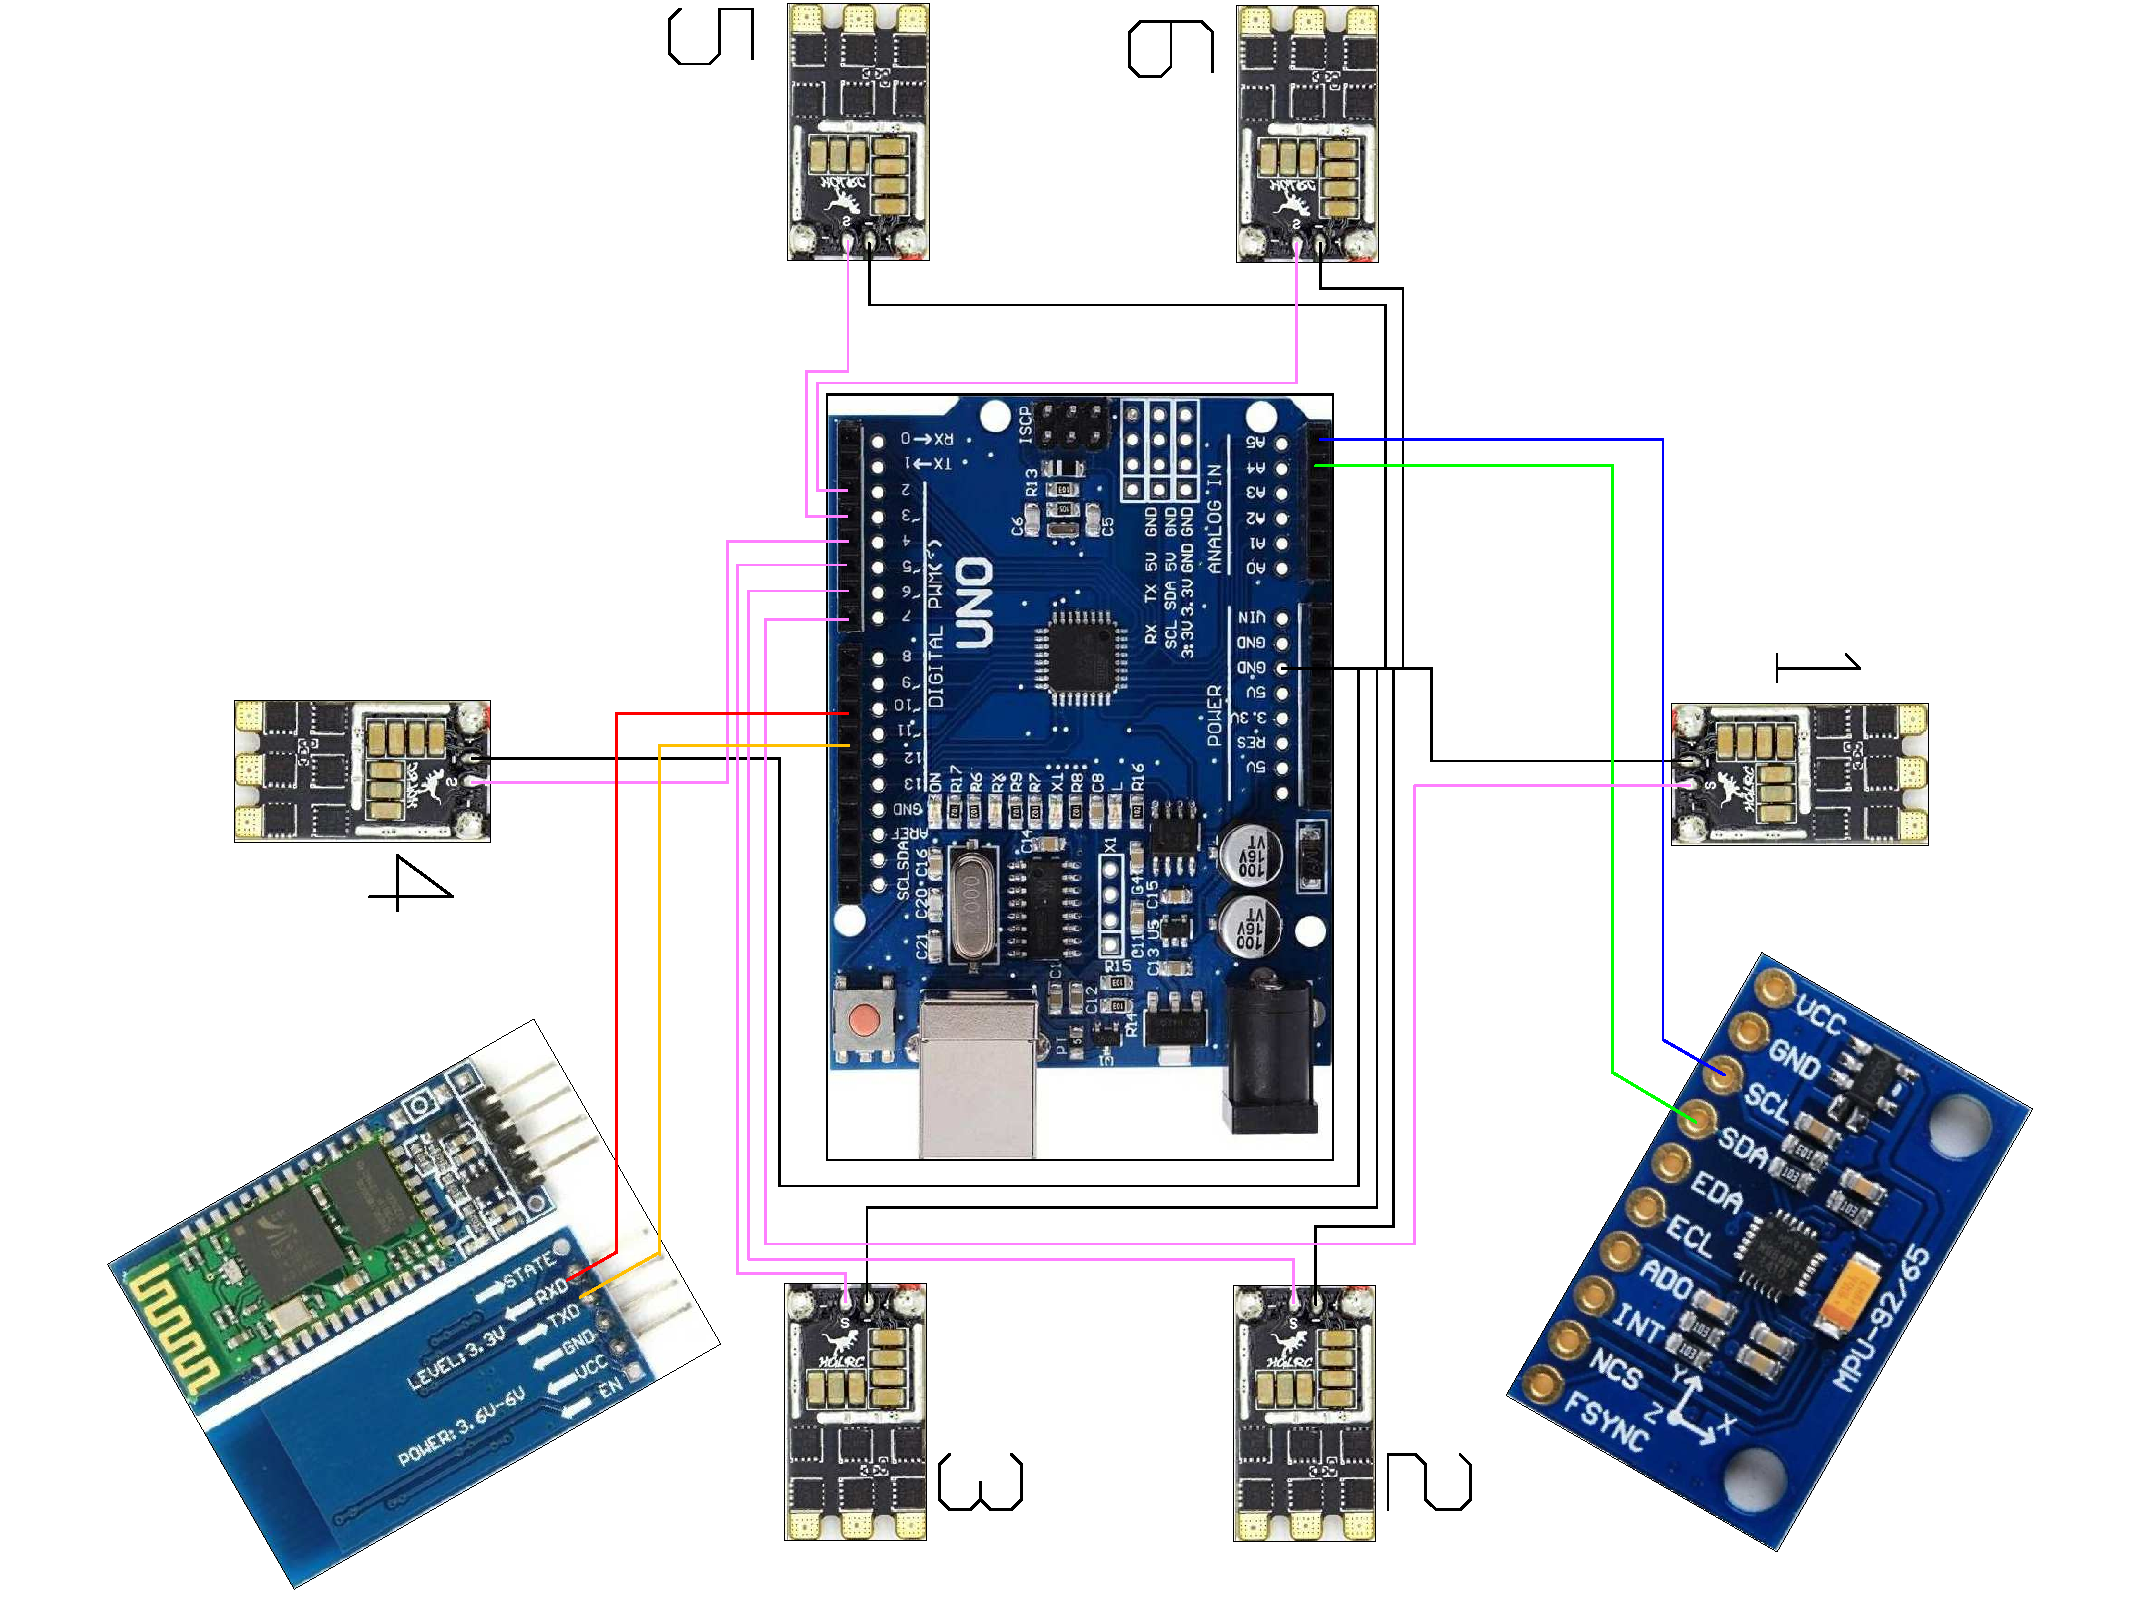
\includegraphics[width=12cm,angle=90]{pictures/flyctrl.pdf}
	\caption{Schéma zapojení Létajícího kontroléru}
\end{figure}

\section{Překážkový kontrolér} 
Vstup: 6x laserový modul\\
Výstup: Navigační kontrolér\\

Překážkový kontrolér má za úkol zabranit kolizi drona s cizím objektem. Laserové moduly jsou nasměrovány do směrů pohybu drona podle úhlů pitch a roll a jsou nastaveny na neustálé měření vzdáleností. Pokud v blízskosi dronu bude cizí objekt kontrolér pošle zprávu o existují překážce navigačnímu kontroléru a její poloze.\\

\begin{figure}[h]
	\centering
	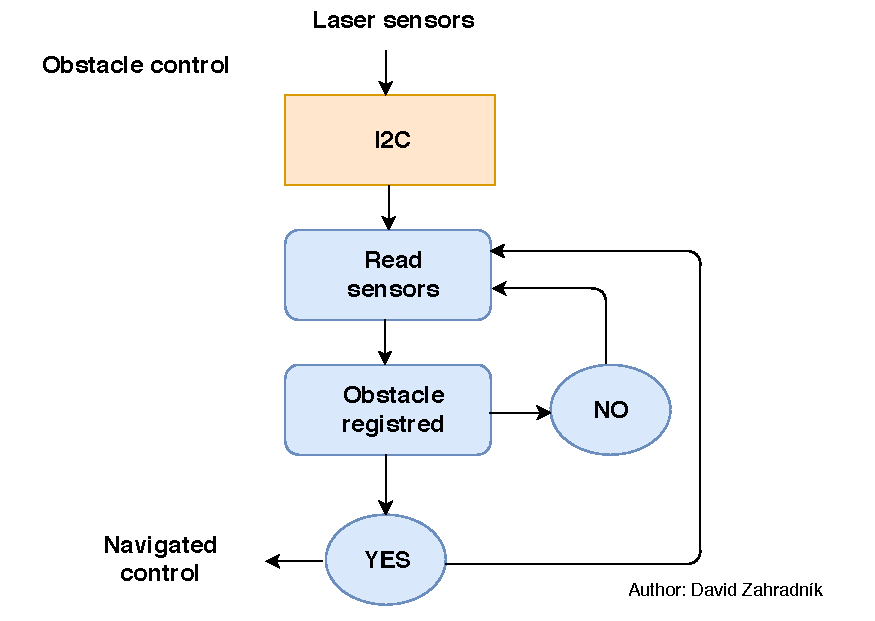
\includegraphics[width=18cm]{pictures/ObstacleDiagram.pdf}
	\caption{Diagram algoritmu překážkového kontroléru}
\end{figure}

\begin{figure}[h]
	\centering
	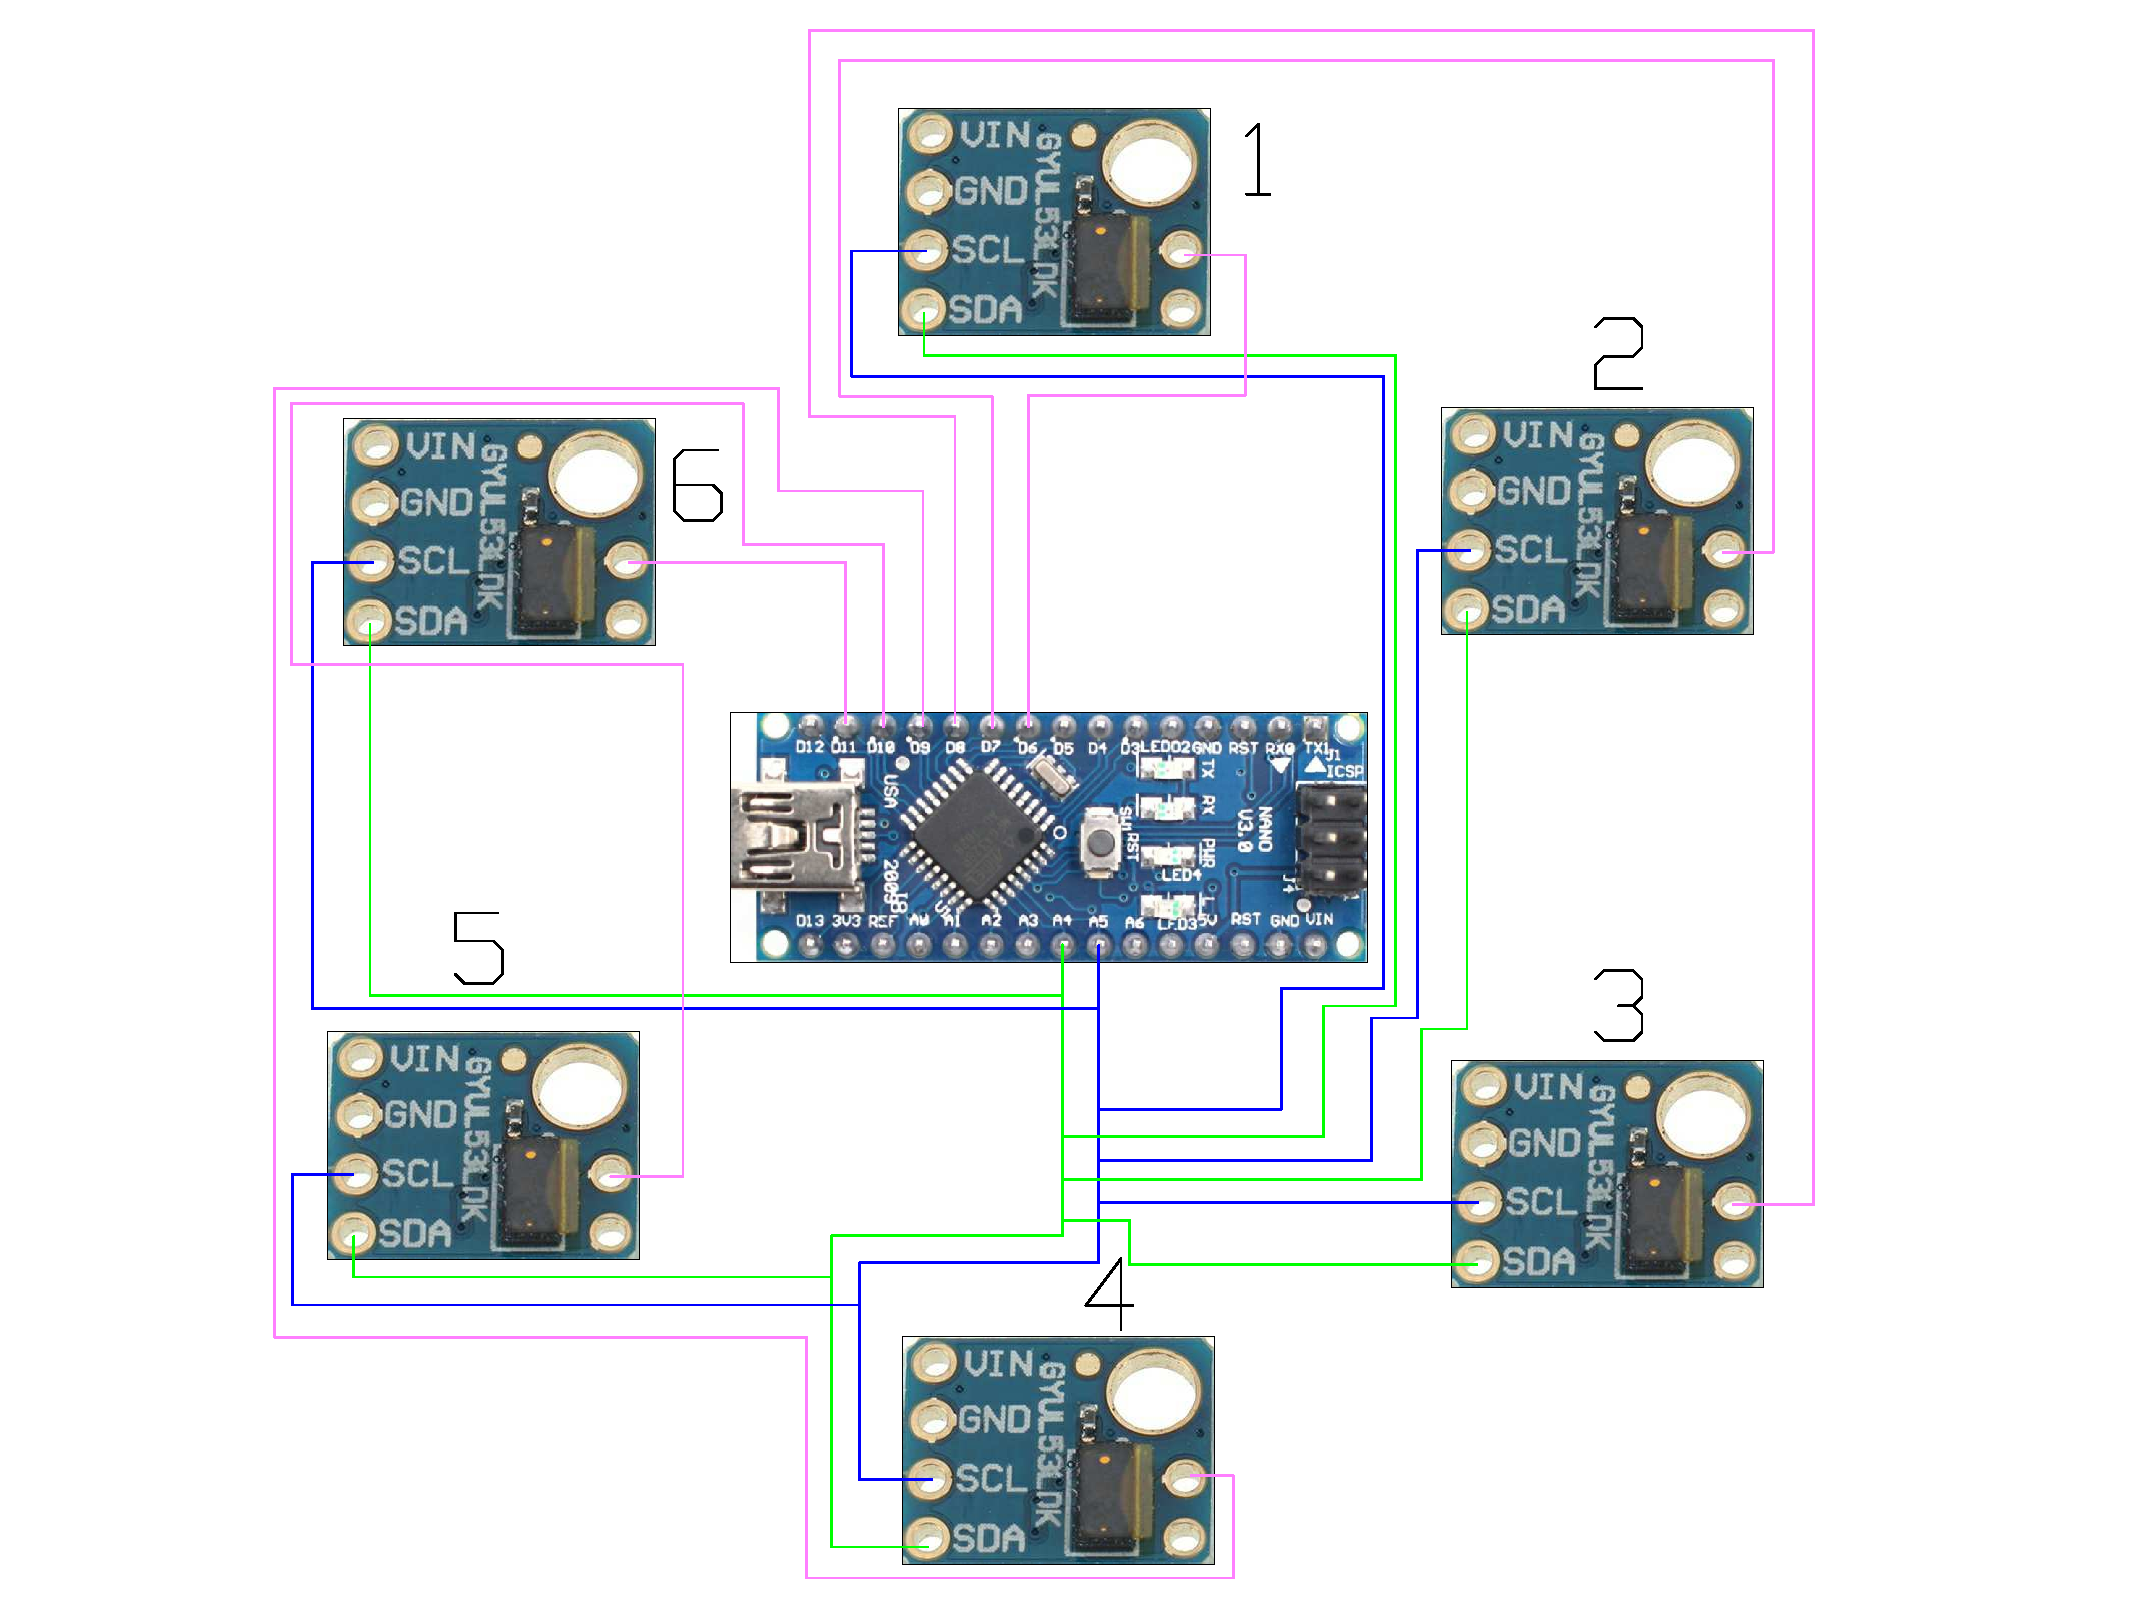
\includegraphics[width=12cm]{pictures/obstacle.pdf}
	\caption{Schéma zapojení Překážkového kontroléru}
\end{figure}

\begin{figure}[h]
	\centering
	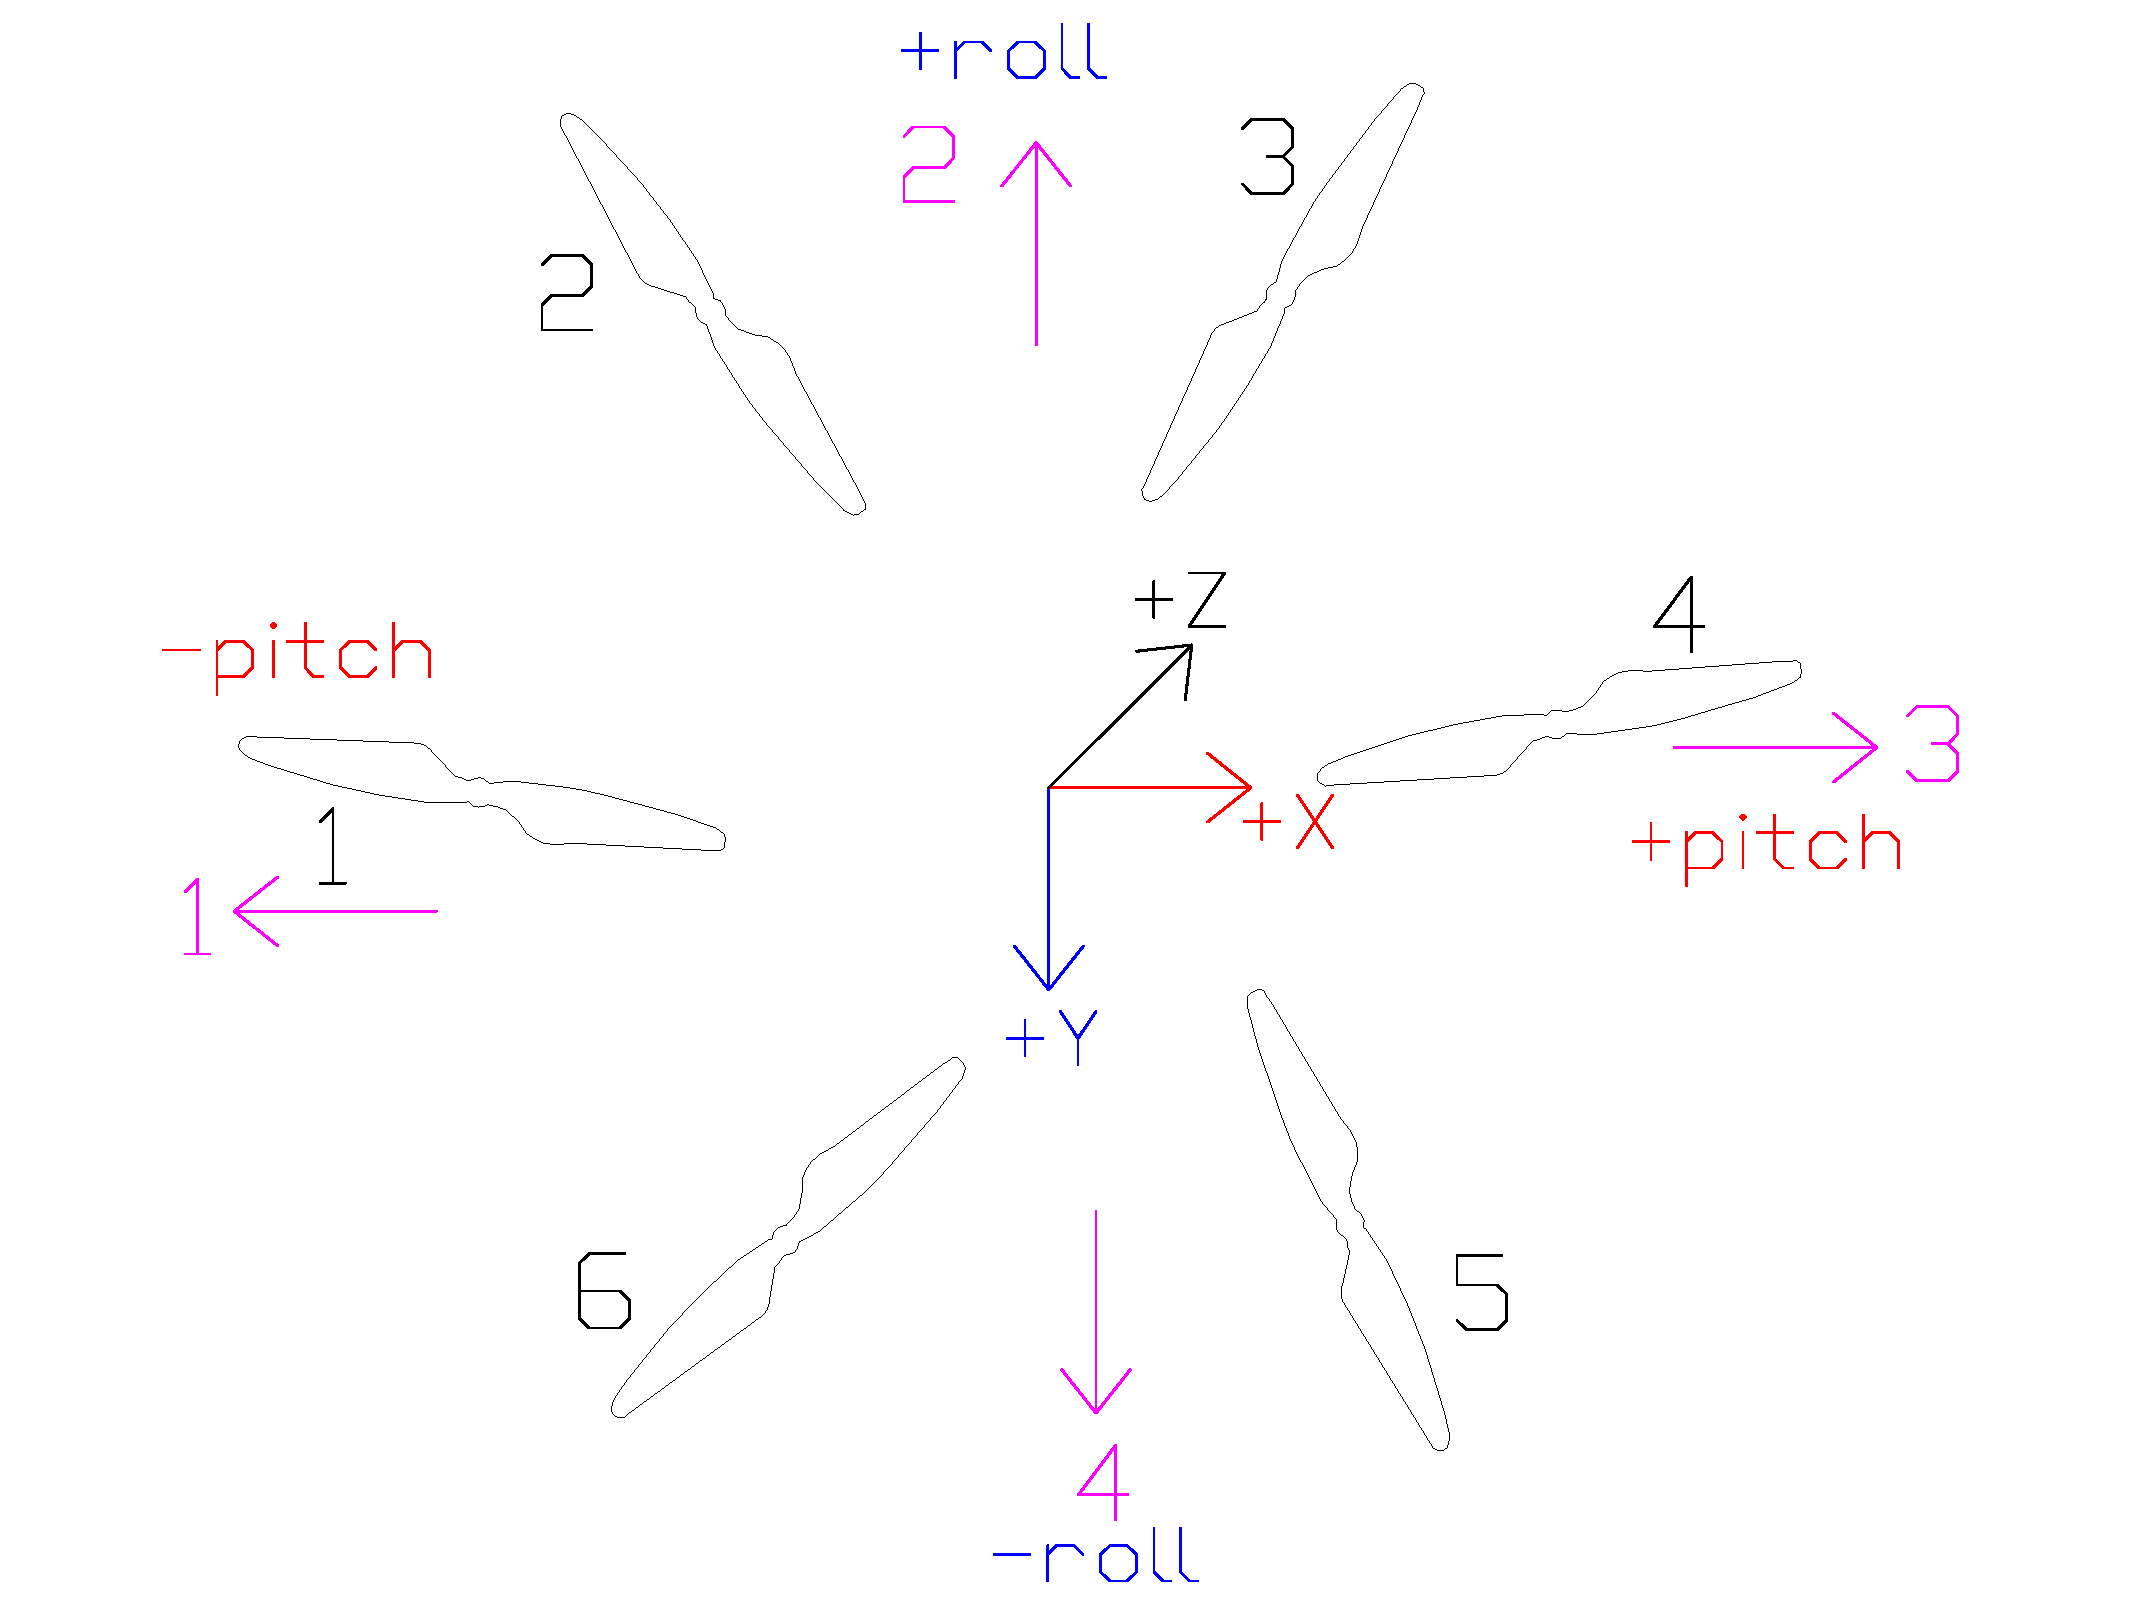
\includegraphics[width=10cm]{pictures/obstacle_teo.pdf}
	\caption{Schéma zpráv o cizím objektu}
\end{figure}

\begin{tabbing}
	+/- ~ \= uhel ~~~ \= zprava ~
	\= 34 \kill
	\bfseries +/- \>
	\bfseries Úhel \>
	\bfseries Zpráva \\
	+\> roll \> 2  \\
	-\> roll \> 4  \\
	-\> pitch \> 1  \\
    +\> pitch \> 3  \\
\end{tabbing}

\section{Navigační kontrolér} 
Vstup: Rádio, Bluetooth, Barometr, GNSS, Překážkový kontrolér\\
Výstup: Létající kontrolér\\

Navigační kontrolér složí ke komunikaci s ovládacím zařízením, sběru dat z gnss, barometru a překážkového kontroléru, vyhodnocení polohy a v závislosti na tom všem ovládat letající kontrolér pro pohyb drona.\\

\begin{figure}[h]
	\centering
	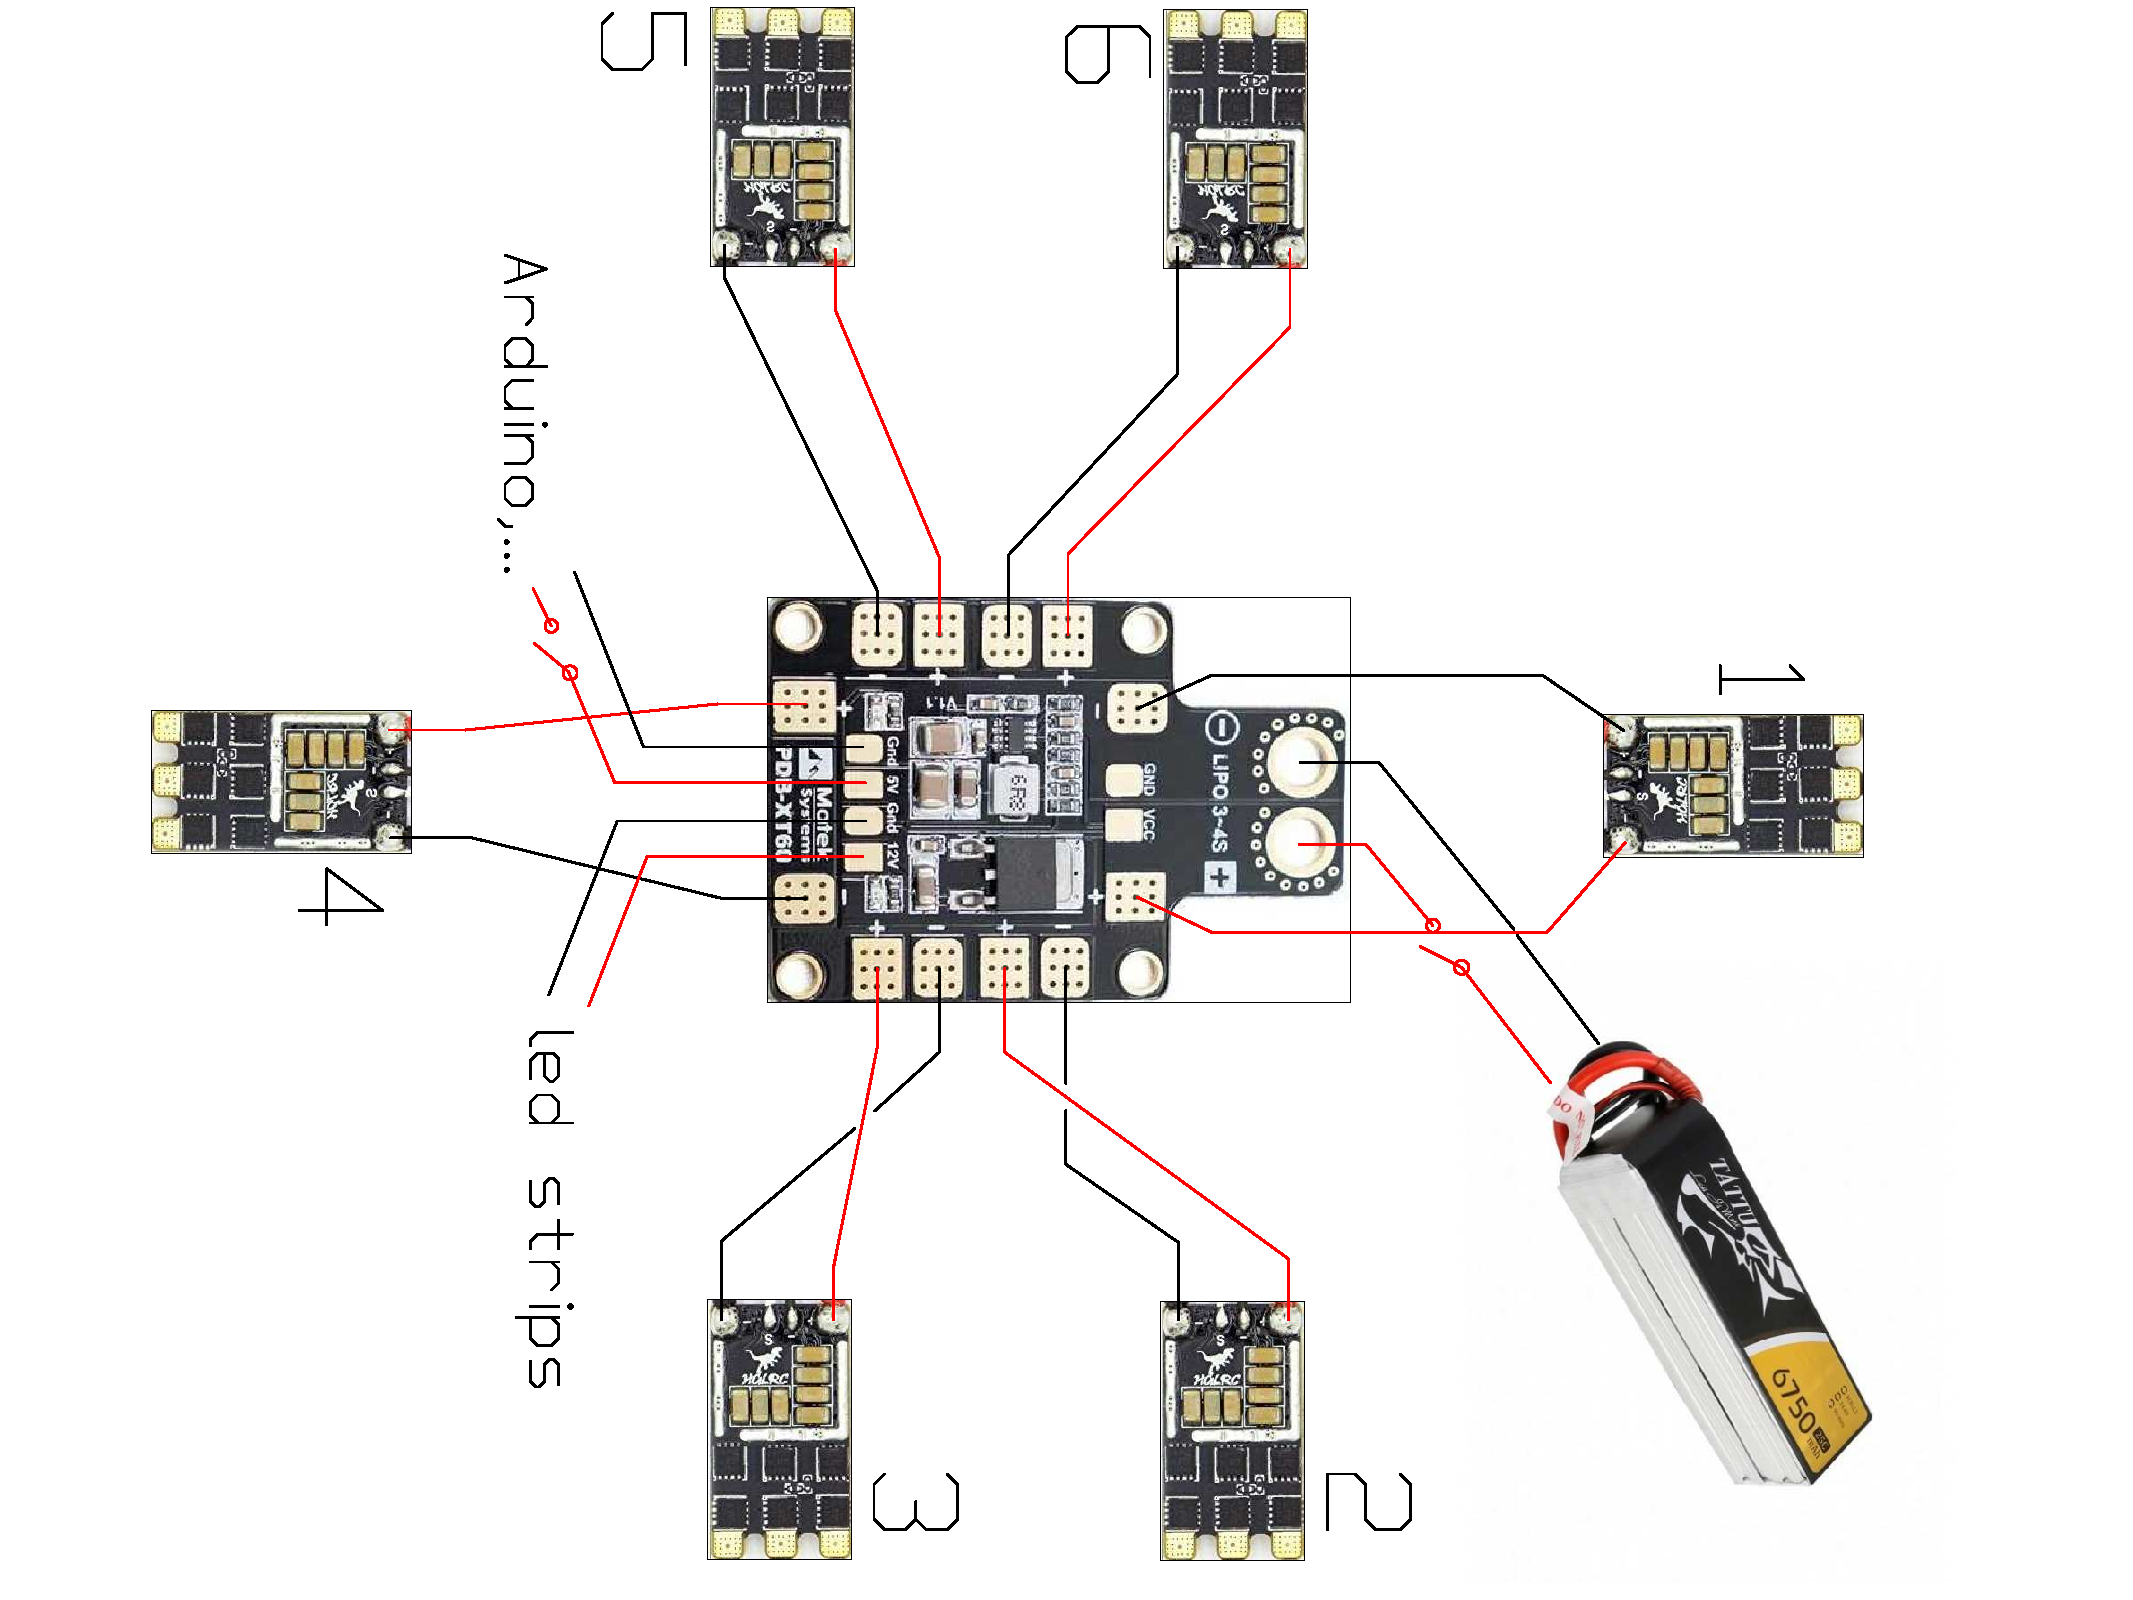
\includegraphics[width=10cm, angle=90]{pictures/pdb_com.pdf}
	\caption{Schéma zapojení napájení motorů}
\end{figure}

\begin{figure}[h]
	\centering
	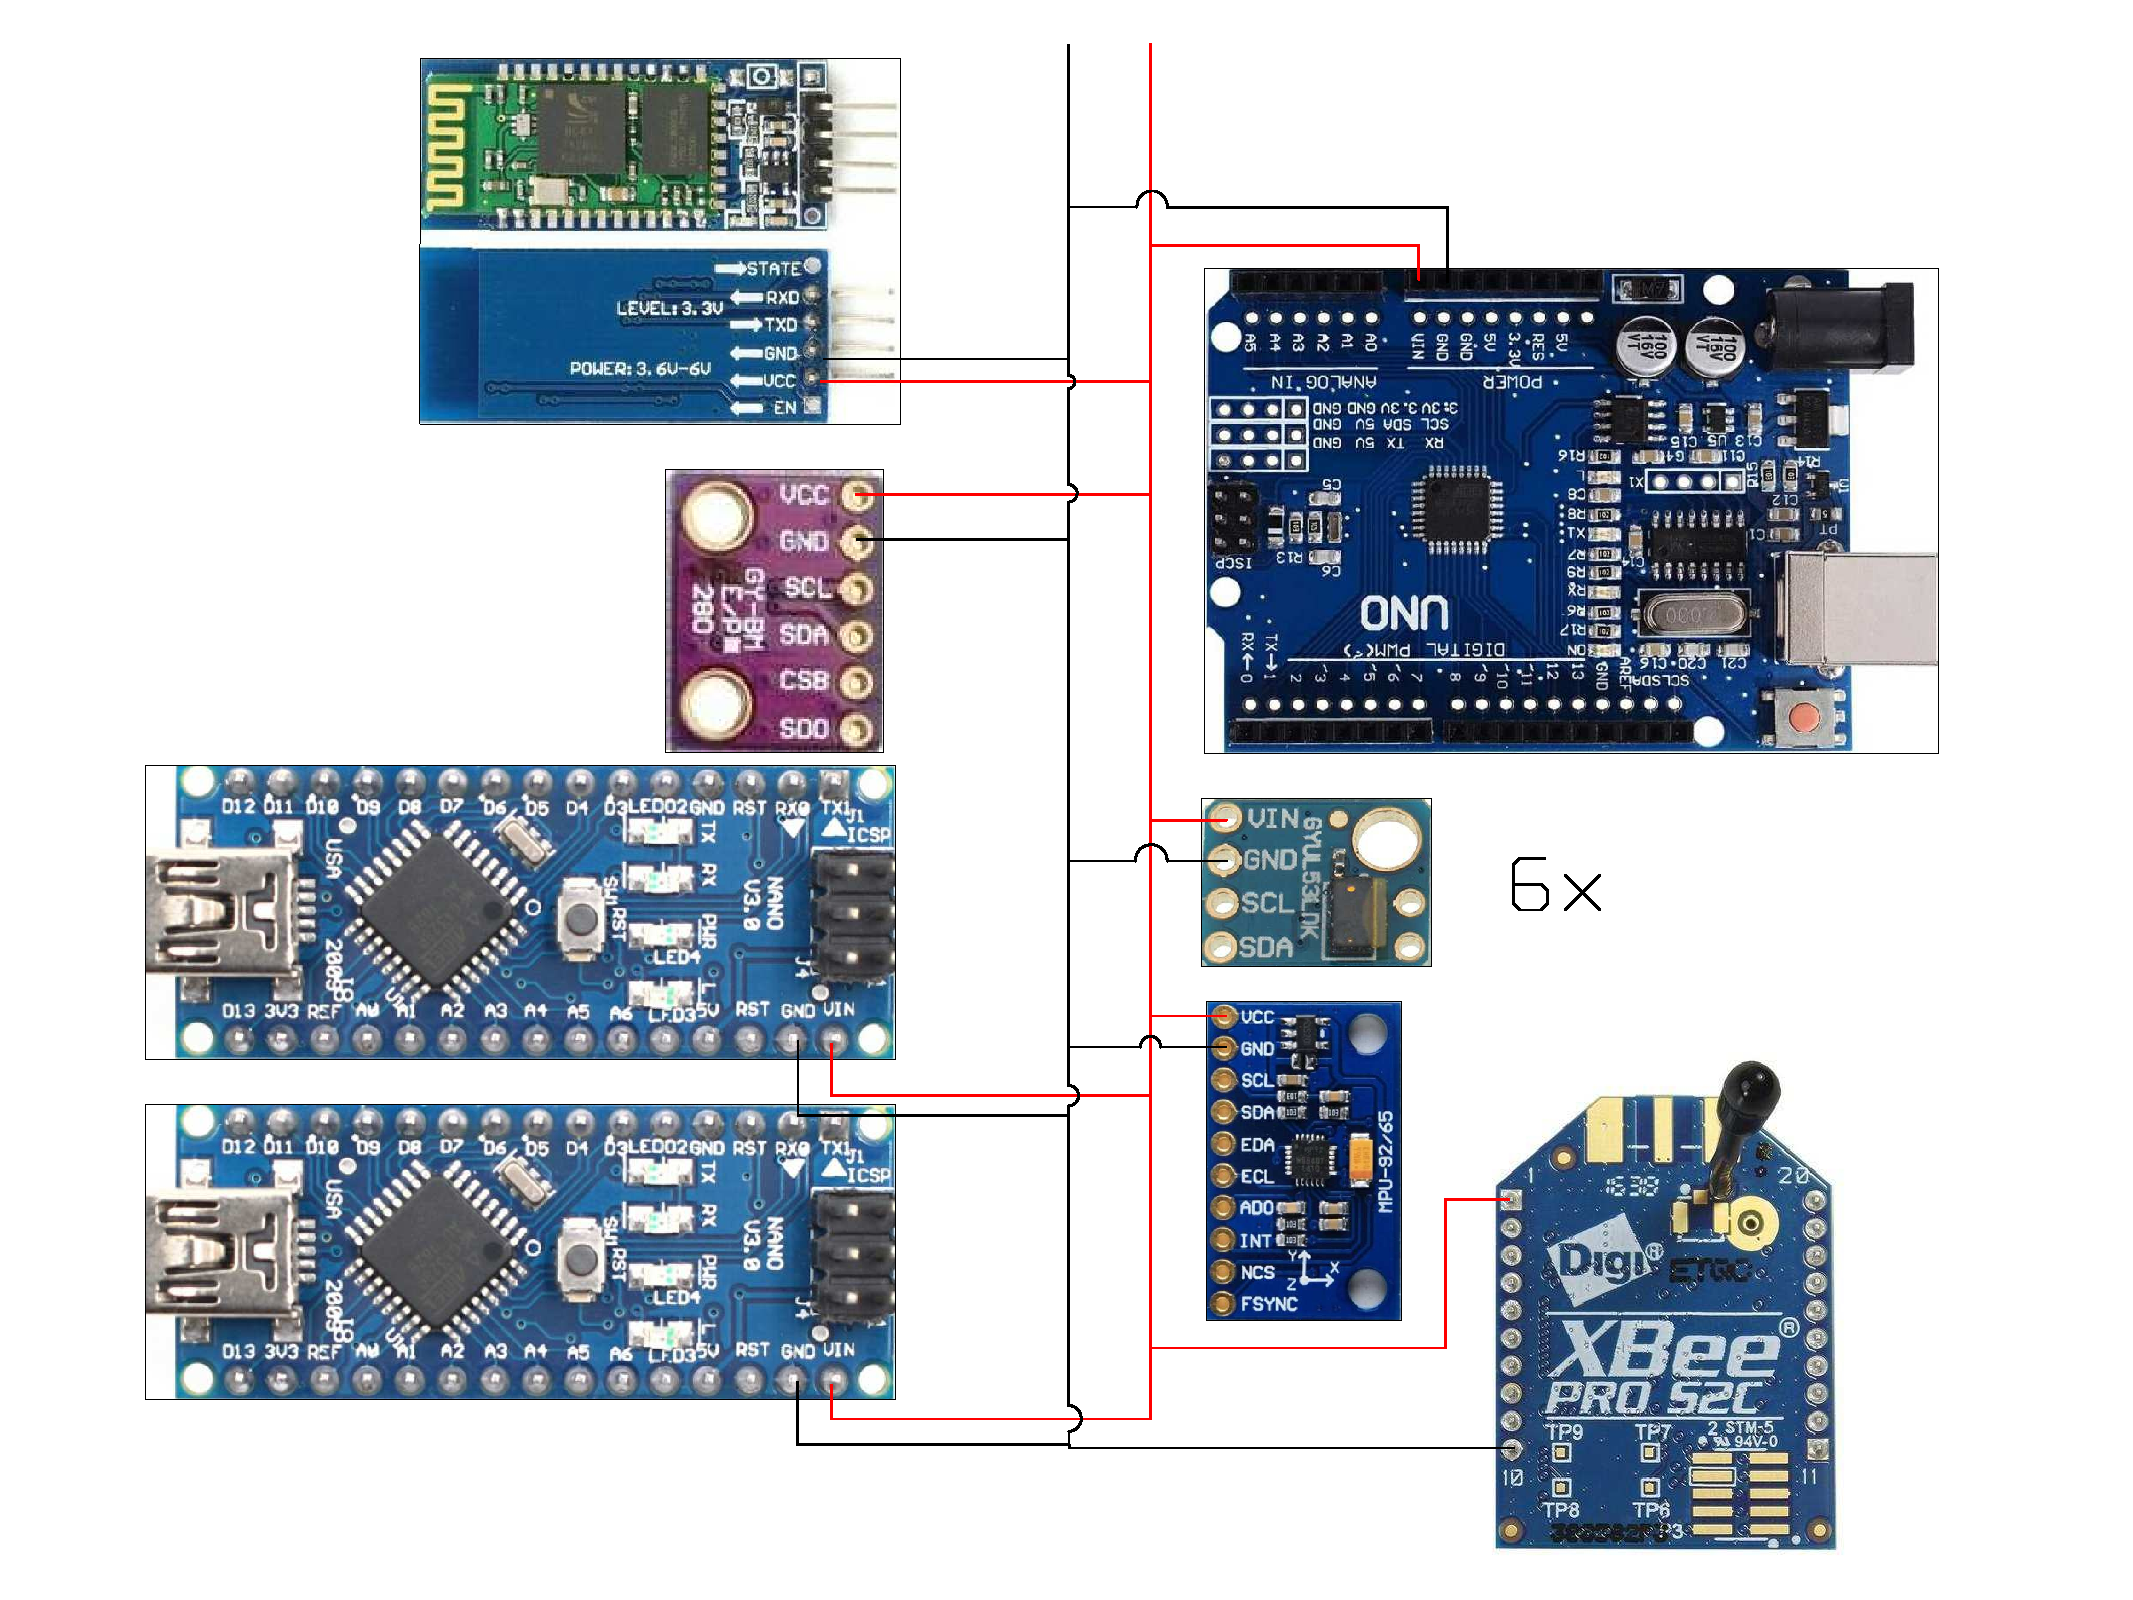
\includegraphics[width=10cm]{pictures/pdb_ardu.pdf}
	\caption{Schéma zapojení napájení Arduina a modulů}
\end{figure}

